\documentclass[11pt,a4paper]{article}

% ----- PACKAGES -----
\usepackage[utf8]{inputenc}
\usepackage[T1]{fontenc}
\usepackage{mathpazo}
\usepackage{amsmath,amssymb,bm}
\usepackage{geometry}
\usepackage{xcolor}
\usepackage{booktabs}
\usepackage[many]{tcolorbox}
\usepackage{titlesec}
\usepackage{enumitem}
\usepackage{graphicx}
\usepackage{caption}
\usepackage{tikz}
\usetikzlibrary{calc,arrows.meta,positioning}
\usepackage{hyperref}

\geometry{top=1.0in, bottom=1.0in, left=1.0in, right=1.0in}

\definecolor{TitleBlue}{RGB}{26, 61, 109}
\definecolor{LabGreen}{RGB}{44, 110, 73}
\definecolor{TaskBg}{RGB}{243, 246, 250}
\definecolor{CheckBg}{RGB}{238, 246, 240}
\definecolor{HintBg}{RGB}{248, 246, 240}

\hypersetup{colorlinks=true, linkcolor=TitleBlue, urlcolor=TitleBlue}

\titleformat{\section}{\large\bfseries\color{TitleBlue}}{\thesection}{0.6em}{}
\titleformat{\subsection}{\bfseries\color{TitleBlue}}{\thesubsection}{0.6em}{}
\captionsetup{font=small, labelfont={bf,color=TitleBlue}, textfont=it}
\setlist{itemsep=2pt, topsep=3pt}

\newtcolorbox{taskbox}{
    enhanced, breakable, colback=TaskBg, colframe=TitleBlue!55,
    boxrule=0.6pt, arc=1.2mm, left=8pt, right=8pt, top=5pt, bottom=6pt,
    title={\textbf{Tasks}}, fonttitle=\small\bfseries, coltitle=white,
    boxed title style={colback=TitleBlue!55, sharp corners},
    attach boxed title to top left={yshift=-2mm, xshift=6pt}
}
\newtcolorbox{checkbox}{
    enhanced, breakable, colback=CheckBg, colframe=LabGreen,
    boxrule=0.6pt, arc=1.2mm, left=8pt, right=8pt, top=5pt, bottom=6pt,
    title={\textbf{Checkpoint}}, fonttitle=\small\bfseries, coltitle=white,
    boxed title style={colback=LabGreen, sharp corners},
    attach boxed title to top left={yshift=-2mm, xshift=6pt}
}
\newtcolorbox{hintbox}{
    enhanced, breakable, colback=HintBg, colframe=gray!55,
    boxrule=0.5pt, arc=1.2mm, left=8pt, right=8pt, top=4pt, bottom=5pt
}

% A small helper for the per-exercise time budget chip.
\newcommand{\budget}[1]{\hfill{\normalfont\small\colorbox{TitleBlue!10}{\textcolor{TitleBlue}{\,$\approx$ #1\,}}}}

\title{\vspace{-2.2em}\textbf{\LARGE Shape Servoing of Deformable Objects}\\[0.3em]
\Large Hands-on Lab Session}
\author{Companion lab to the notes \emph{An Introduction to Jacobian-Based Shape Servoing}}
\date{Estimated duration: 2.5--3 hours}

\begin{document}
\maketitle
\vspace{-1em}

% ===========================================================
\section*{Overview}

In this lab we will develop a shape controller that brings a deformable object to a
desired target shape, without assuming any mechanical model of the object. The object is a
planar elastic rod held at both ends by two grippers, each with three degrees of freedom
(DoF). The grippers impose end-effector (EE) poses on the rod; the rod settles into an
equilibrium shape; a perception step samples a small set of points along it; and the
controller adjusts the EE poses, step by step, until those sampled points reach a predefined
target configuration.

The controller's actuation space is the six-dimensional end-effector pose vector
$\mathbf{r}=[x_L,y_L,\theta_L,x_R,y_R,\theta_R]^\top$, and its feature space is the
ten-dimensional sampled-point vector $\mathbf{s}=[x_1,y_1,\dots,x_5,y_5]^\top$. The method
centres on the \emph{interaction Jacobian} $\mathbf{J}$, the local linear map relating a
gripper motion $\dot{\mathbf{r}}$ to the change $\dot{\mathbf{s}}$ it produces in the measured shape. Across the exercises we will
estimate it from data, invert it to close a control loop, keep it accurate as the rod
deforms, and analyse the three characteristic ways in which the loop fails. Together, the
exercises build a complete (if minimal) data-driven shape-servoing pipeline that runs in
two phases (Figures~\ref{fig:loop-offline} and~\ref{fig:loop-online}). In the
\emph{offline} phase, the robots run a short exploration sequence and a least-squares fit
produces an initial Jacobian estimate $\hat{\mathbf{J}}^{(0)}$ (Exercise~3). In the \emph{online}
phase, the controller turns the shape error $\mathbf{e}=\mathbf{s}^{*}-\mathbf{s}$ into an action $\Delta\mathbf{r}$; the
robots apply it as the EE pose $\mathbf{r}$ holding the rod; the rod settles into a new true state
$\mathbf{x}$; a perception step maps $\mathbf{x}$ to the measured features $\mathbf{s}$; and a Broyden update keeps
$\hat{\mathbf{J}}$ current (Exercise~4).

\begin{figure}[h!]
\centering
\resizebox{\linewidth}{!}{%
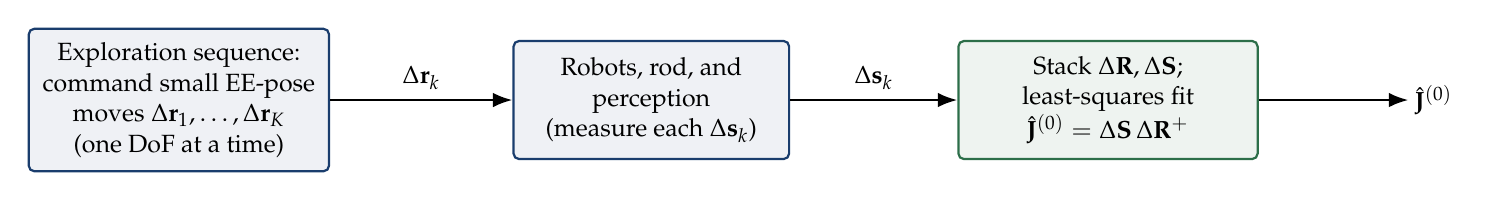
\begin{tikzpicture}[>=Latex, font=\small,
  blk/.style={draw=TitleBlue, line width=0.8pt, rounded corners=2pt, fill=TitleBlue!7,
              align=center, inner sep=5pt, minimum height=1.5cm, minimum width=3.5cm},
  fit/.style={draw=LabGreen, line width=0.8pt, rounded corners=2pt, fill=LabGreen!8,
              align=center, inner sep=5pt, minimum height=1.5cm, minimum width=3.8cm},
  sig/.style={->, line width=0.9pt}]
  \node[blk] (cal) at (0,0)    {Exploration sequence:\\command small EE-pose\\moves $\Delta\mathbf{r}_1,\dots,\Delta\mathbf{r}_K$\\(one DoF at a time)};
  \node[blk] (sys) at (6.0,0)  {Robots, rod, and\\perception\\(measure each $\Delta\mathbf{s}_k$)};
  \node[fit] (fit) at (11.8,0) {Stack $\Delta\mathbf{R},\Delta\mathbf{S}$;\\least-squares fit\\$\hat{\mathbf{J}}^{(0)}=\Delta\mathbf{S}\,\Delta\mathbf{R}^{+}$};
  \draw[sig] (cal) -- node[above]{$\Delta\mathbf{r}_k$} (sys);
  \draw[sig] (sys) -- node[above]{$\Delta\mathbf{s}_k$} (fit);
  \draw[sig] (fit.east) -- ++(1.9,0) node[right, inner sep=2pt]{$\hat{\mathbf{J}}^{(0)}$};
\end{tikzpicture}}
\caption{\textbf{Offline initialisation.} The robots run an exploration sequence, moving
one EE degree of freedom at a time; each commanded move $\Delta\mathbf{r}_k$ and its measured
feature response $\Delta\mathbf{s}_k$ are stacked into $\Delta\mathbf{R},\Delta\mathbf{S}$ and fit by least
squares to give the initial Jacobian estimate $\hat{\mathbf{J}}^{(0)}$.}
\label{fig:loop-offline}
\end{figure}

\begin{figure}[h!]
\centering
\resizebox{\linewidth}{!}{%
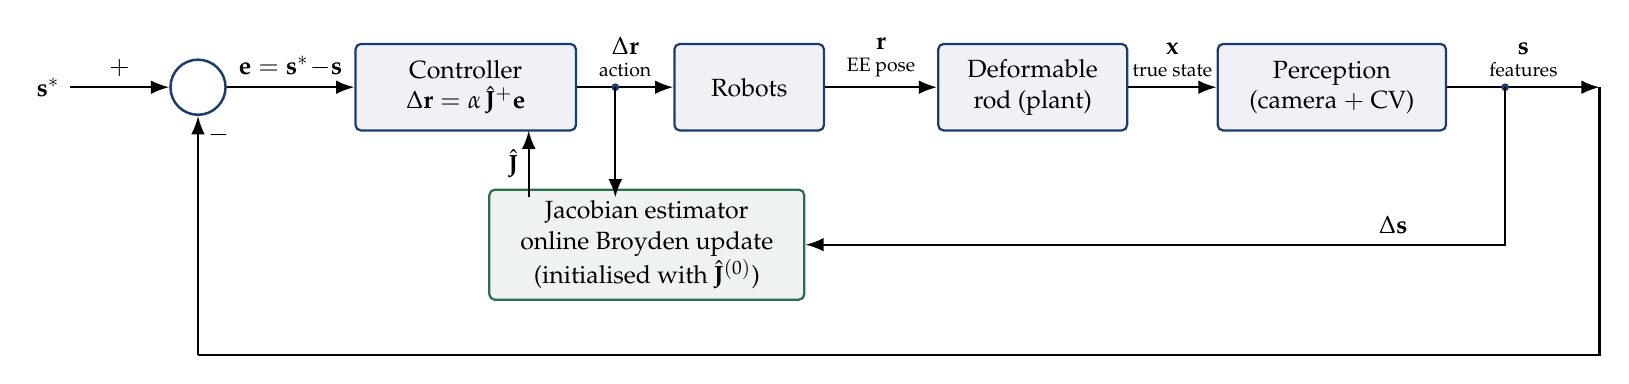
\begin{tikzpicture}[>=Latex, font=\small,
  blk/.style={draw=TitleBlue, line width=0.8pt, rounded corners=2pt, fill=TitleBlue!7,
              align=center, inner sep=4pt, minimum height=1.1cm},
  est/.style={draw=LabGreen, line width=0.8pt, rounded corners=2pt, fill=LabGreen!8,
              align=center, inner sep=4pt, minimum height=1.2cm, minimum width=4.0cm},
  sum/.style={draw=TitleBlue, line width=0.9pt, circle, minimum size=7mm, inner sep=0pt},
  sig/.style={->, line width=0.8pt},
  lab/.style={above, align=center, font=\small}]

  \node[sum] (sum) at (0,0) {};
  \node[blk, minimum width=2.8cm] (ctrl) at (3.4,0)  {Controller\\$\Delta\mathbf{r}=\alpha\,\hat{\mathbf{J}}^{+}\mathbf{e}$};
  \node[blk, minimum width=1.9cm] (rob)  at (7.0,0)  {Robots};
  \node[blk, minimum width=2.4cm] (rod)  at (10.6,0) {Deformable\\rod (plant)};
  \node[blk, minimum width=2.9cm] (perc) at (14.4,0) {Perception\\(camera $+$ CV)};

  \node (ref) at (-1.9,0) {$\mathbf{s}^{*}$};
  \draw[sig] (ref)  -- node[pos=0.5, above, font=\small]{$+$} (sum);
  \draw[sig] (sum)  -- node[lab]{$\mathbf{e}=\mathbf{s}^{*}\!-\!\mathbf{s}$} (ctrl);
  \draw[sig] (ctrl) -- node[lab]{$\Delta\mathbf{r}$\\[-3pt]{\scriptsize action}} (rob);
  \draw[sig] (rob)  -- node[lab]{$\mathbf{r}$\\[-3pt]{\scriptsize EE pose}} (rod);
  \draw[sig] (rod)  -- node[lab]{$\mathbf{x}$\\[-3pt]{\scriptsize true state}} (perc);
  \coordinate (sout) at (17.8,0);
  \draw[sig] (perc) -- node[lab]{$\mathbf{s}$\\[-3pt]{\scriptsize features}} (sout);

  \draw[line width=0.8pt] (sout) -- (17.8,-3.4) -- (0,-3.4);
  \draw[sig] (0,-3.4) -- node[pos=0.92, right, font=\small]{$-$} (sum);

  \node[est] (est) at (5.7,-2.0) {Jacobian estimator\\online Broyden update\\(initialised with $\hat{\mathbf{J}}^{(0)}$)};
  \fill[TitleBlue] (5.3,0) circle (1.4pt);
  \fill[TitleBlue] (16.6,0) circle (1.4pt);
  \draw[sig] (4.2,-1.4) -- node[left, pos=0.5, font=\small]{$\hat{\mathbf{J}}$} (4.2,-0.55);
  \draw[sig] (5.3,0) -- (5.3,-1.4);
  \draw[sig] (16.6,0) -- (16.6,-2.0) -- node[above, pos=0.16, font=\small]{$\Delta\mathbf{s}$} (est.east);
\end{tikzpicture}}
\caption{\textbf{Online control loop.} The forward path (blue) turns the shape error
$\mathbf{e}=\mathbf{s}^{*}-\mathbf{s}$ into an action $\Delta\mathbf{r}$, which the robots apply as the EE pose $\mathbf{r}$ holding
the rod; the rod settles to a true state $\mathbf{x}$, which the perception block maps to the
measured features $\mathbf{s}$, fed back (with a minus sign) to form the next error. The estimator
(green) refines the Jacobian $\hat{\mathbf{J}}$ from $\Delta\mathbf{r}$ and $\Delta\mathbf{s}$, starting from
$\hat{\mathbf{J}}^{(0)}$.}
\label{fig:loop-online}
\end{figure}

\paragraph{How the lab is organised.} The lab is five short scripts, one per exercise,
completed in order: \texttt{ex1\_setup.py}, \texttt{ex2\_representation.py},
\texttt{ex3\_offline\_jacobian.py}, \texttt{ex4\_control\_loop.py}, and
\texttt{ex5\_failure\_modes.py}. Each one \emph{imports} the functions you wrote in the
earlier ones, so the controller is built up step by step and the code stays small. Fill in
the lines marked \texttt{TODO}; the blocks marked ``provided'' (reporting and plotting) are
not edited. The rod physics (\texttt{dlo.py}) and the plotting helpers (\texttt{labviz.py})
are provided too: the rod is a black box that returns the equilibrium shape for any
commanded EE pose. Run a script with, e.g., \texttt{python ex3\_offline\_jacobian.py}; the
figure each exercise should produce is reproduced alongside it below, so you can check your
own result. Exercise~5 is a separate, diagnostic study and can be run on its own.

\begin{checkbox}
\textbf{Before you start (\,$\approx$ 10 min\,).} Create a Python environment and
install the dependencies (\texttt{README.md} gives the per-operating-system
commands):
\begin{quote}\small\ttfamily
python -m pip install -r requirements.txt
\end{quote}
Then change into \texttt{code/} and check that the libraries and the rod back-end
import without error:
\begin{quote}\small\ttfamily
cd code\\
python -c "import numpy, scipy, matplotlib, dlo, labviz"
\end{quote}
You will work through \texttt{ex1\_setup.py} to \texttt{ex5\_failure\_modes.py} in order.
The figures appear when you run a script; if no display is available, each exercise still
writes its figure to a \texttt{.png} file next to the script.
\end{checkbox}

\paragraph{Notation (used throughout).}
Following the control convention, $n$ is the feature-space (output) dimension and $m$ the
actuation (input) dimension. The rod's true physical state is $\mathbf{x}$, its equilibrium configuration; a
perception step maps $\mathbf{x}$ to the feature vector $\mathbf{s}\in\mathbb{R}^{n}$ ($n=2P=10$, from $P=5$ sampled
points stacked as $[x_1,y_1,\dots,x_P,y_P]$), which the controller uses.
$\mathbf{r}\in\mathbb{R}^{m}$ ($m=6$) is the end-effector (EE) pose we command (two 3-DoF gripper
poses stacked). $\mathbf{s}^{*}$ is the target and $\mathbf{e}=\mathbf{s}^{*}-\mathbf{s}$ the shape error.
$\mathbf{J}\in\mathbb{R}^{n\times m}$ is the true interaction Jacobian ($\dot{\mathbf{s}} = \mathbf{J}\dot{\mathbf{r}}$), and
$\hat{\mathbf{J}}$ is the estimate we actually use. $\mathbf{J}^{+}$ denotes the Moore--Penrose pseudo-inverse.

\paragraph{Objectives.} After this lab you should be able to:
\begin{enumerate}[label=(\alph*)]
    \item explain what a shape feature vector is and how its choice changes which
    deformations the controller can measure;
    \item estimate an interaction Jacobian from motion data and characterise its
    rank and conditioning from the singular values;
    \item implement a pseudo-inverse shape controller and a Broyden online
    update;
    \item recognise the numerical signatures of the three failure modes of the
    loop.
\end{enumerate}

\vspace{0.4em}\hrule

% ===========================================================
\section{The shape-servoing problem \budget{15 min}}

\textbf{Goal.} Exercise 1 defines the controller's actuation space and feature space,
obtains the current and target feature vectors, and computes the shape error that the
later feedback controller will reduce. We define a nominal EE pose $\mathbf{r}$ and a
target pose $\mathbf{r}^{*}$; for each we solve the rod equilibrium and sample it to obtain the
feature vectors $\mathbf{s}$ and $\mathbf{s}^{*}$; and we compute the shape error $\mathbf{e}=\mathbf{s}^{*}-\mathbf{s}$ and its norm
$\lVert\mathbf{e}\rVert$.

\begin{taskbox}
In \texttt{ex1\_setup.py}:
\begin{enumerate}
    \item Choose a nominal grasp and a reachable target grasp (each gripper pose is
    $[x,y,\theta]$); pick a target that visibly moves or bends the rod, and try a few.
    \item Complete \texttt{sampled\_points} (solve the rod, then sample it), and form the
    feature vectors $\mathbf{s},\mathbf{s}^{*}$ and the error $\mathbf{e}=\mathbf{s}^{*}-\mathbf{s}$.
\end{enumerate}
\end{taskbox}

\begin{checkbox}
The script reports $\dim \mathbf{r} = 6$, $\dim \mathbf{s} = 10$, and the initial error
$\lVert\mathbf{e}\rVert$ (its value depends on the grasps you chose; the example in
Figure~\ref{fig:ex1} gives $\approx 1.3$). Each arrow links a measured point to the
target it must reach.
\end{checkbox}

\begin{figure}[h!]
\centering
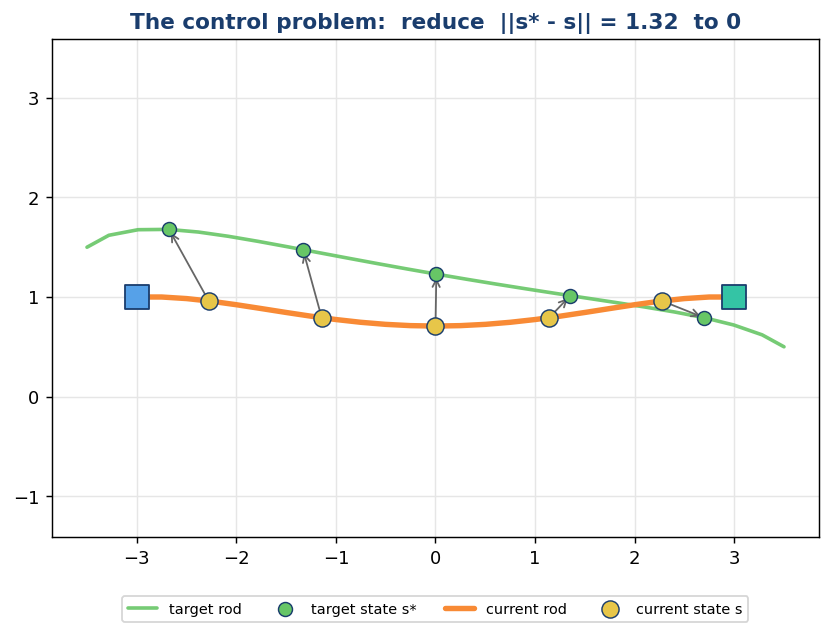
\includegraphics[width=0.62\linewidth]{figs/ex1_setup.png}
\caption{Expected output. The control problem: bring the measured state (yellow)
onto the target state (green).}
\label{fig:ex1}
\end{figure}

% ===========================================================
\section{Choosing the shape representation \budget{25 min}}

\textbf{Goal.} The feature vector $\mathbf{s}$ is a design choice, and different choices
retain different information about the rod. We compare three representations of the same
$P$ sampled points $\mathbf{p}_1,\dots,\mathbf{p}_P$, and test how each responds to a \emph{rigid
transformation} (a translation and a rotation applied to the whole rod, without deforming
it):
\begin{itemize}
    \item \textbf{point coordinates} $\mathbf{s}=[x_i,y_i]$: absolute positions;
    \item \textbf{edge vectors} $\mathbf{e}_i = \mathbf{p}_{i+1}-\mathbf{p}_i$: invariant to
    translation;
    \item \textbf{curvature} $\kappa_i=\theta_{i+1}-\theta_i$ (turning angle
    between consecutive edges): invariant to any rigid motion.
\end{itemize}

\begin{taskbox}
In \texttt{ex2\_representation.py}:
\begin{enumerate}
    \item Implement \texttt{rep\_points}, \texttt{rep\_edges}, \texttt{rep\_curvature}, and
    \texttt{rigid\_motion} (rotate the points about their centroid, then translate).
    \item Set \texttt{FEATURE} to the representation the controller will use in Exercises~3
    and~4. The comparison and plot are provided.
\end{enumerate}
\end{taskbox}

\begin{checkbox}
After a translation, $\lVert\Delta\mathbf{s}\rVert$ should be large for point
coordinates and (numerically) zero for both edge vectors and curvature. After a
translation \emph{and} a rotation, only curvature should stay at zero
(Figure~\ref{fig:ex2}). Explain \emph{why} edge vectors are unchanged by a
translation but change under a rotation.
\end{checkbox}

\begin{figure}[h!]
\centering
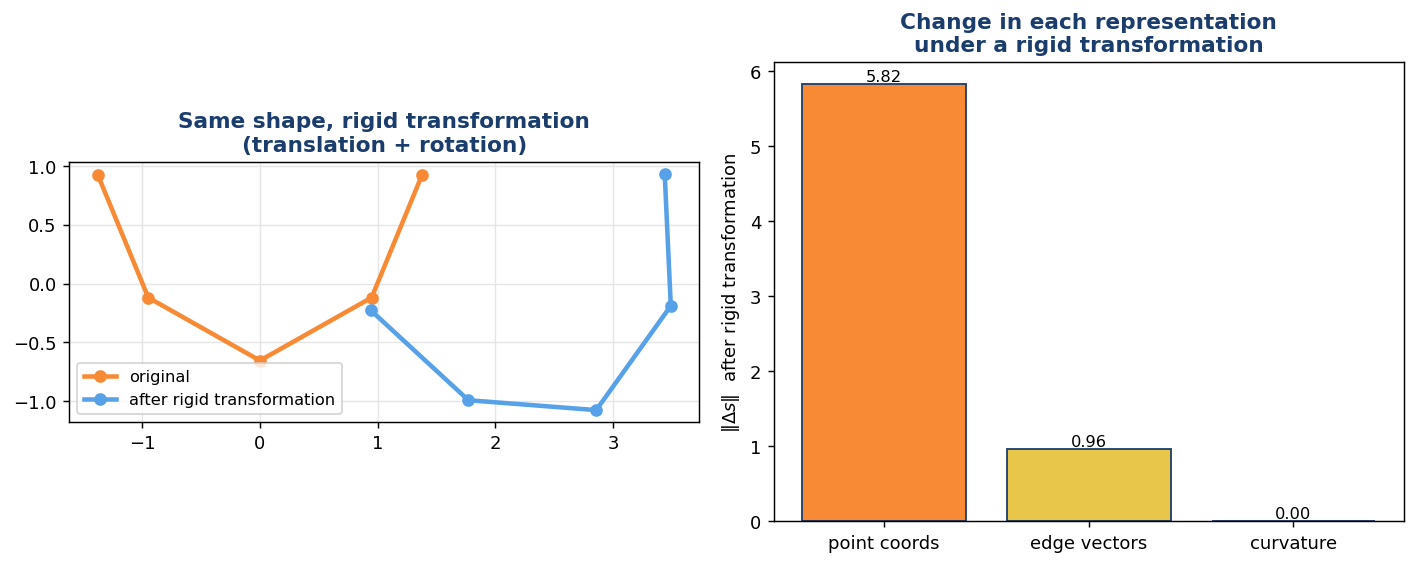
\includegraphics[width=0.9\linewidth]{figs/ex2_representation.png}
\caption{Expected output. The same shape under a rigid transformation; only the
representations invariant to a given motion report $\lVert\Delta\mathbf{s}\rVert\approx 0$.}
\label{fig:ex2}
\end{figure}

\begin{hintbox}\small
The three values have different units (metres vs.\ radians), so do not compare
their magnitudes across representations. Read each only as ``zero'' or
``non-zero''.
\end{hintbox}

% ===========================================================
\section{Offline Jacobian estimation \budget{40 min}}

\textbf{Goal.} The controller never has a model of the rod, so it never computes a ``true''
Jacobian. Instead it \emph{estimates} the interaction Jacobian from data: we move each
gripper DoF a little, gather the input changes $\Delta\mathbf{R}\,(m\times K)$ and the output
changes $\Delta\mathbf{S}\,(n\times K)$, and fit the single $\hat{\mathbf{J}}^{(0)}$ that best maps them by
least squares,
\[
    \hat J^{(0)} \;=\; \Delta S\,\Delta R^{+}.
\]
We then read its rank and conditioning from the singular values
$\sigma_1\ge\dots\ge\sigma_6$: the \emph{rank} is how many independent shape directions the
grippers can produce; the \emph{manipulability} $w=\prod_i\sigma_i$ is the overall actuation
capacity; and the \emph{condition number} $\kappa=\sigma_{\max}/\sigma_{\min}$ is the ratio
between the most and least responsive directions.

\begin{taskbox}
In \texttt{ex3\_offline\_jacobian.py}:
\begin{enumerate}
    \item Choose the exploration moves (\texttt{EXPLORE\_AMP}, \texttt{EXPLORE\_FRACS}).
    \item Complete \texttt{offline\_jacobian}: gather $\Delta\mathbf{R},\Delta\mathbf{S}$ from the
    exploration moves, then regress $\hat{\mathbf{J}}^{(0)}=\Delta\mathbf{S}\,\Delta\mathbf{R}^{+}$.
    \item In \texttt{svd\_metrics}, compute the rank, manipulability $w$, and condition
    number $\kappa$ from the singular values.
\end{enumerate}
\end{taskbox}

\begin{checkbox}
With point-coordinate features and the suggested moves, the offline fit residual is
$\lVert\Delta\mathbf{S}-\hat{\mathbf{J}}^{(0)}\Delta\mathbf{R}\rVert\approx 0.31$, and the estimate has full column
rank ($\mathrm{rank}=6$), manipulability $w\approx 0.20$, and condition number
$\kappa\approx 17$. The figure shows $\hat{\mathbf{J}}^{(0)}$ as a heat-map and its six singular
values (Figure~\ref{fig:ex3}).
\end{checkbox}

\begin{figure}[h!]
\centering
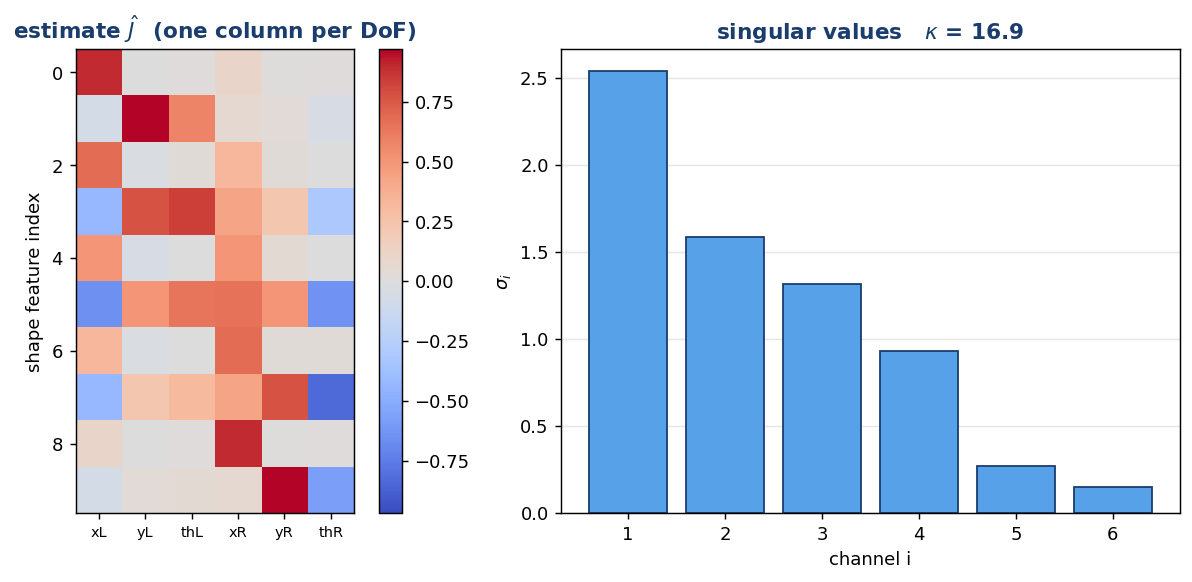
\includegraphics[width=0.92\linewidth]{figs/ex3_jacobian.png}
\caption{Expected output. The offline Jacobian estimate $\hat{\mathbf{J}}^{(0)}$ as a heat-map (one
column per gripper DoF) and its six singular values.}
\label{fig:ex3}
\end{figure}

% ===========================================================
\section{Closing the loop with an online update \budget{40 min}}

\textbf{Goal.} We put the estimate to work. Starting from the offline $\hat{\mathbf{J}}^{(0)}$ of
Exercise~3, the controller closes the loop with the pseudo-inverse step
\[
    \Delta r \;=\; \alpha\, \hat J^{+}(s^{*}-s),\qquad
    \hat J^{+}=(\hat J^{\top}\hat J)^{-1}\hat J^{\top},
\]
and, because a fixed estimate drifts as the rod deforms, it refreshes $\hat{\mathbf{J}}$ after every
step with the Broyden rank-one update
\[
    \hat J \;\leftarrow\; \hat J + \frac{(\Delta s - \hat J\,\Delta r)\,\Delta r^{\top}}{\Delta r^{\top}\Delta r}.
\]

\begin{hintbox}\small
\textbf{The control loop (high level).} From the nominal grasp, repeat until the error is
small: (1)~measure $\mathbf{s}$ and form $\mathbf{e}=\mathbf{s}^{*}-\mathbf{s}$, and stop if $\lVert\mathbf{e}\rVert$ is small;
(2)~take the step $\Delta\mathbf{r}=\alpha\,\hat{\mathbf{J}}^{+}\mathbf{e}$ and apply it ($\mathbf{r}\leftarrow \mathbf{r}+\Delta\mathbf{r}$);
(3)~measure the new shape and the change $\Delta\mathbf{s}$; (4)~update $\hat{\mathbf{J}}$ with the Broyden
rule, and record $\lVert\mathbf{e}\rVert$. The small gain $\alpha=0.05$ makes the decay smooth and
easy to read; try $\alpha=0.3$ to compare.
\end{hintbox}

\begin{taskbox}
In \texttt{ex4\_control\_loop.py}:
\begin{enumerate}
    \item Implement the Broyden update in \texttt{broyden\_update}.
    \item Complete the control loop in \texttt{main()}, following the pseudocode above. It
    starts from the offline estimate $\hat{\mathbf{J}}^{(0)}$ imported from Exercise~3.
\end{enumerate}
\end{taskbox}

\begin{checkbox}
With the Broyden update on, the loop drives the error from $\approx 1.3$ down to the
tolerance in about $100$ iterations (Figure~\ref{fig:ex4}). Now set \texttt{USE\_BROYDEN = False}
and re-run: the fixed offline estimate drifts as the rod deforms, so the same loop
converges much more slowly. Updating $\hat{\mathbf{J}}$ online is what keeps convergence fast.
\end{checkbox}

\begin{figure}[h!]
\centering
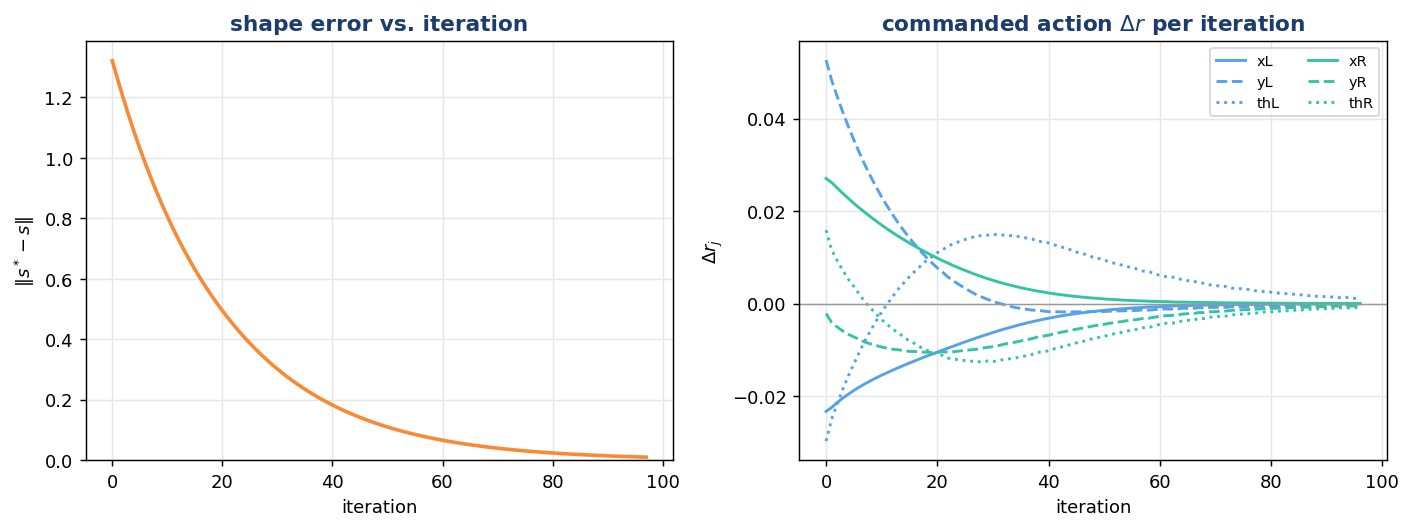
\includegraphics[width=0.9\linewidth]{figs/ex4_estimation.png}
\caption{Expected output. The control loop driving the shape to the target: the error
$\lVert \mathbf{s}^{*}-\mathbf{s}\rVert$ decays to zero (left) while the commanded action $\Delta\mathbf{r}$ shrinks
as the error vanishes (right).}
\label{fig:ex4}
\end{figure}

% ===========================================================
\section{The three ways the loop fails \budget{35 min}}

\textbf{Goal.} A shape-servoing loop relies on three conditions holding at once.
Each one can fail, and each failure has a distinct numerical signature. In this exercise we
reproduce all three. The conditioning analysis uses the rod's \texttt{true\_jacobian}
oracle, a Jacobian the controller never has, used here only to reveal the mechanics.

\begin{enumerate}
    \item \textbf{Controllability (taut state).} Pull the rod straight by
    increasing the gripper separation. Some gripper motions stop producing any
    shape change, so the Jacobian loses rank from its \emph{columns}:
    $\sigma_{\min}\to 0$, $w\to 0$, $\kappa\to\infty$.
    \item \textbf{Observability (insensitive feature).} Move one gripper up and
    the other down by the same amount. The rod clearly deforms, but a symmetric
    scalar feature (the midpoint height) does not move: the feature map is
    insensitive to this deformation (a rank loss from the \emph{rows}).
    \item \textbf{Mechanical instability (buckling).} Compress the rod by
    reducing the gripper separation. At a critical point the smallest eigenvalue
    of the elastic-energy Hessian crosses zero; the straight equilibrium becomes
    unstable and the rod snaps. No finite linear $\mathbf{J}$ describes that jump.
\end{enumerate}

\begin{taskbox}
In \texttt{ex5\_failure\_modes.py} (it reuses your \texttt{svd\_metrics} from Exercise~3):
\begin{enumerate}
    \item In \texttt{taut\_curve}, build the straight grasp at each separation, get its
    Jacobian from \texttt{rod.true\_jacobian}, and read $\sigma_{\min}$, $w$ and $\kappa$.
    \item In \texttt{observability\_curve}, build the antisymmetric motion (left gripper up
    by $\delta$, right gripper down by $\delta$).
    \item In \texttt{buckling\_curve}, query the rod for the smallest energy-Hessian
    eigenvalue at each separation (\texttt{rod.straight\_min\_eig}).
\end{enumerate}
\end{taskbox}

\begin{checkbox}
The figures (Figure~\ref{fig:ex5}) should show $\kappa$ rising from about $17$ to $117$
as the rod is pulled taut; the full state growing while the midpoint feature
stays flat at zero; and the energy-Hessian eigenvalue crossing zero near a
gripper separation of $6.0$ (the rod's rest length), marking the onset of buckling.
\end{checkbox}

\begin{figure}[h!]
\centering
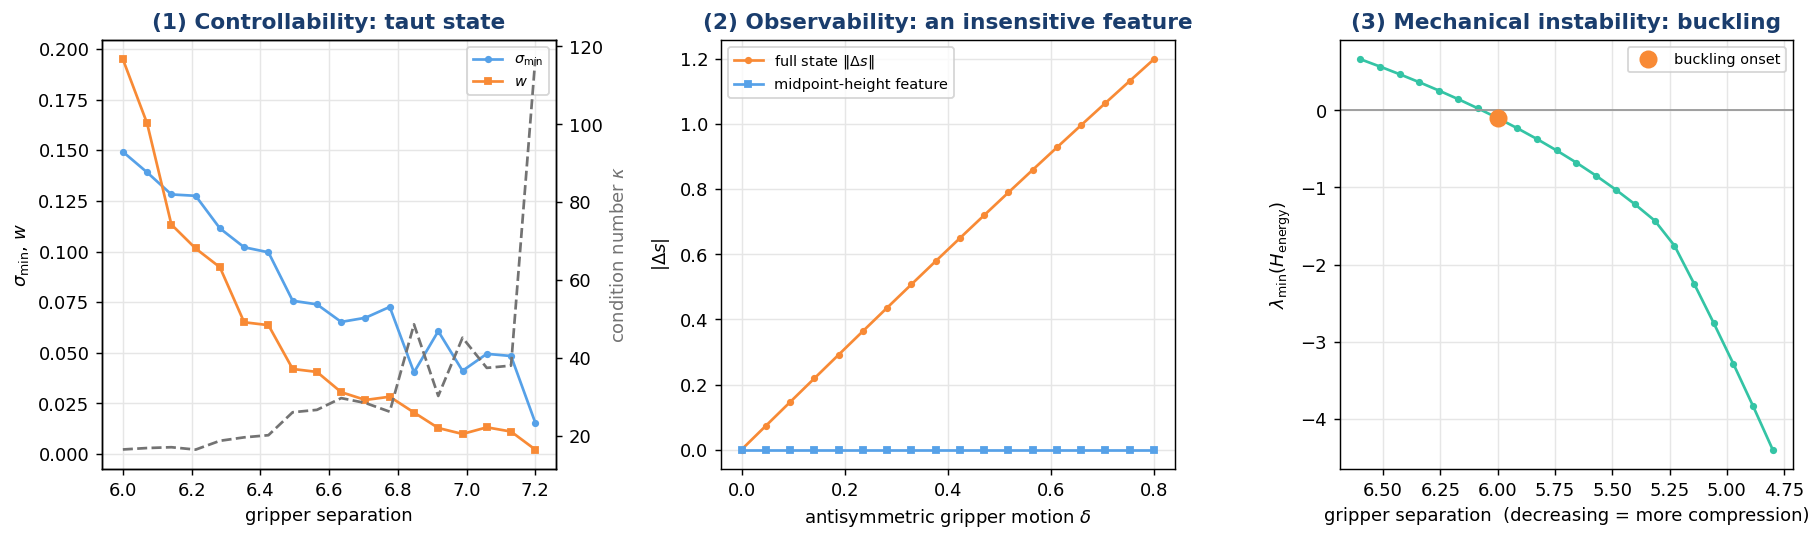
\includegraphics[width=\linewidth]{figs/ex5_failure_modes.png}
\caption{Expected output. Left to right: the taut-state collapse, the symmetric
feature insensitive to the deformation, and the buckling eigenvalue crossing zero.}
\label{fig:ex5}
\end{figure}

% ===========================================================
\section*{Wrapping up}

Across the five exercises we have built every block of a model-free shape-servoing loop:
a feature representation, a least-squares Jacobian estimate kept current online, a
pseudo-inverse controller, and the diagnostics that reveal when the loop is about to fail.
The same structure extends to richer features and real
perception: what changes is how $\mathbf{s}$ is measured and how $\hat{\mathbf{J}}$ is estimated, not the
structure of the loop itself.

\paragraph{Optional extensions.} Any one of the following: (i) set \texttt{FEATURE} to
curvature in Exercise~2 and see how the estimate and the convergence change; (ii) make the
rod less stiff (\texttt{Rod(k\_bend=1.0)}) and compare the convergence; (iii) in
Exercise~4, plot $\lVert\hat{\mathbf{J}}-\mathbf{J}_{\text{true}}\rVert$ (using \texttt{rod.true\_jacobian})
over the iterations to follow how the estimate tracks the true Jacobian.

\end{document}
